\documentclass[border=10pt]{standalone}
\usepackage{tikz}
\usetikzlibrary{automata, positioning, arrows.meta}

\begin{document}
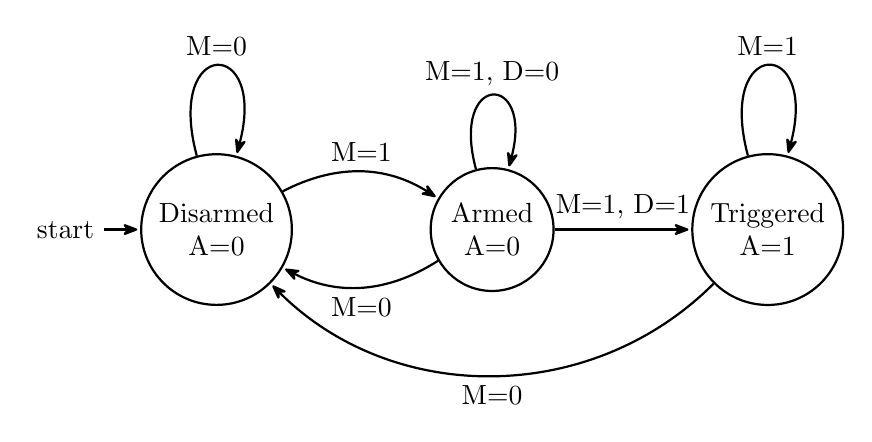
\begin{tikzpicture}[shorten >=1pt, node distance=3.5cm, on grid, auto, >={Stealth[round]}, thick]
    % Nodes
    % S0: Disarmed, A=0
    \node[state, initial] (s0) [align=center] {Disarmed\\A=0};
    
    % S1: Armed, A=0
    \node[state] (s1) [right=of s0, align=center] {Armed\\A=0};
    
    % S2: Triggered, A=1
    \node[state] (s2) [right=of s1, align=center] {Triggered\\A=1};

    % Transitions
    \path[->]
        % S0 transitions
        (s0) edge [loop above] node {M=0} (s0)
             edge [bend left] node {M=1} (s1)
             
        % S1 transitions
        (s1) edge [bend left] node {M=0} (s0)
             edge [loop above] node {M=1, D=0} (s1)
             edge node {M=1, D=1} (s2)
             
        % S2 transitions
        (s2) edge [bend left=45] node [below] {M=0} (s0)
             edge [loop above] node {M=1} (s2);

\end{tikzpicture}
\end{document}
